\section{Discussion}
\label{sec:discussion}

We have presented CHAODA, an ensemble of six algorithms that use the map of the underlying manifold produced by CLAM\@.
The six individual algorithms are simple to implement on top of CLAM and, when combined into an ensemble, often outperform state-of-the-art methods.

CLAM uses the geometric and topological properties of fractal dimension and metric entropy of the data to build a map of the low-dimensional manifold that the data occupy.
CLAM is inspired by the clustering algorithm from CHESS~\cite{ishaq2019clustered}, but differs by the introduction a novel graph-induction approach and a notion of optimal depths, learned via a form of ``meta-machine-learning'' and transfer learning.
CLAM's selection of ``poles'' for partitioning clusters is also more efficient than CHESS.
CHAODA builds on this manifold-mapping framework for anomaly and outlier detection.
Intuitively, we expect CHAODA to perform particularly well when the data lie on an ``interesting'' manifold, and to perform merely average when the data derive from an easily-described distribution (or ``boring'' manifold).
Just as CHESS demonstrated an acceleration of search when the data exhibited \emph{low fractal dimension} and \emph{low metric entropy}, with CHAODA, we see that AUC scores are vastly improved when the data exhibit these properties and often competitive when the data do not exhibit these properties.


% A simple visualization in Figure~\ref{fig:conclusions:umap-embeddings} using UMAP~\cite{mcinnes2018umap} illustrates two different examples; the anomalies in one dataset, where CHAODA outperforms other methods, appear to be at the edges of a complex manifold (though, clearly, the UMAP projection has distorted the manifold) while in another dataset, where most methods perform fairly comparably, the distribution is less interesting and many anomalies are distributed apparently randomly across it.

% \begin{figure*}
%    \centering
%    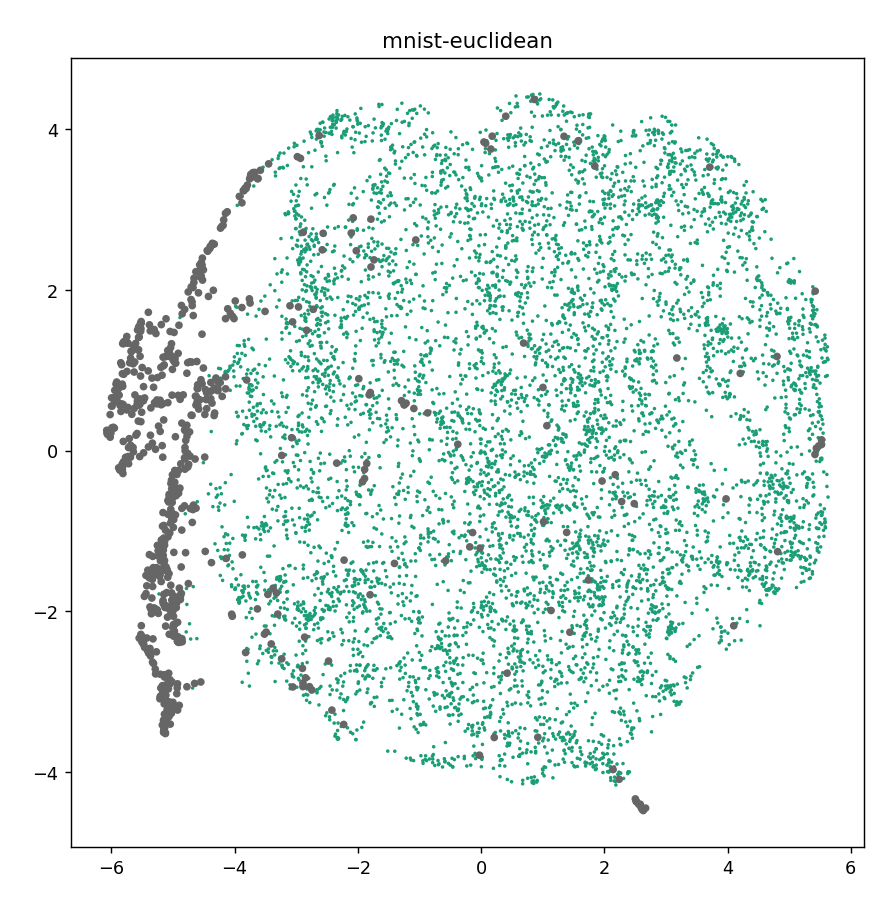
\includegraphics[width=2in]{images/umaps/mnist-euclidean-umap2d.png}
%    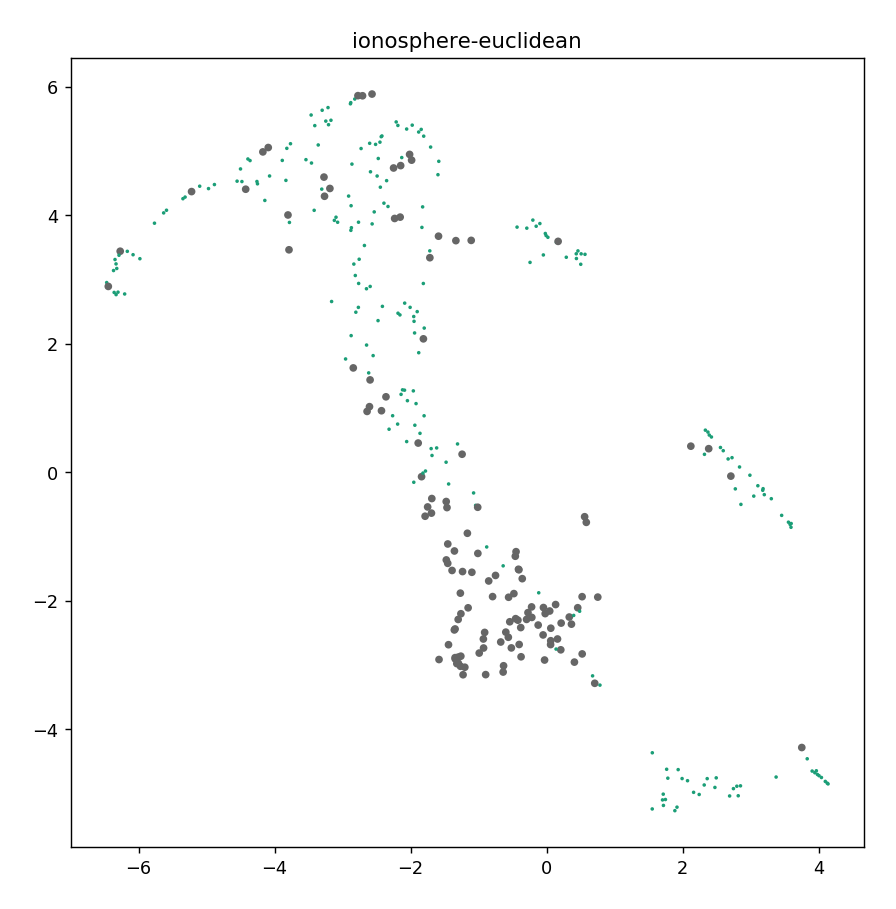
\includegraphics[width=2in]{images/umaps/ionosphere-euclidean-umap2d.png}
%    \caption{UMAP projection of MNIST (left) and Ionosphere (right). Anomalies are in gray. Note that for MNIST, the UMAP projection does not find much structure, though most of the anomalies congregate to one side. For Ionosphere, there is a single main component to the manifold, with two more distant clusters, and anomalies tend to be at the edges of a manifold. Most algorithms perform comparably on MNIST, while CHAODA outperforms others on Ionosphere.}
%    \label{fig:conclusions:umap-embeddings}
% \end{figure*}

% \subsection{Future Directions}
% \label{subsec:discussion:future-directions}


The choice of distance function could have a significant impact on anomaly-detection performance.
In this case, domain knowledge is likely the best way to determine the distance function of choice.
Future work should explore a more diverse collection of domain-appropriate distance functions, such as Wasserstein distance on images, Levenshtein edit distance on strings, and Jaccard distance on the maximal common subgraph of molecular structures.

CHAODA is demonstrably highly effective on high-dimensional datasets, and so may be applied to neural networks.
Using CLAM to map a dataset where each datum represents the activations of a neural network from an input to the neural network, we would expect to detect malicious inputs to neural networks based on the intuition that malicious inputs produce atypical activation patterns.

In conclusion, we have demonstrated that by mapping the manifolds occupied by data, CLAM reveals structure that allows CHAODA to outperform other state-of-the-art approaches to anomaly detection.
